\chapter{Risultati e Conclusioni}

\section{Risultati ottenuti}

Il lavoro ha portato allo sviluppo di una pipeline completa per il taglio
robotizzato di un indumento, dalla percezione all'esecuzione sul manipolatore
reale. Il sistema è stato validato prima in ambiente simulato con Unity e
successivamente sull'UR5, ottenendo l'esecuzione delle traiettorie
pianificate sul robot fisico.

Per quanto riguarda il modulo di visione, la rete YOLOv8n-seg addestrata sul
dataset realizzato ad hoc ha raggiunto sul validation set un
mAP@50 del \textbf{90.3\%} per il rilevamento (box) e del \textbf{56.8\%} per
la segmentazione (maschere). La matrice di confusione evidenzia ottime
prestazioni sul colletto (0.98) e sul fondomaglia (0.91), e una resa leggermente
inferiore sui polsini (0.81). Le prestazioni sulle
maschere sono inferiori a quelle sui box, coerentemente con la natura sottile
degli elementi da segmentare; l'algoritmo di estrazione geometrica ha tuttavia permesso di ricavare in modo robusto la
linea media delle cuciture, sufficiente per la generazione dei riferimenti.

\begin{figure}[htbp]
    \centering
    % Prima immagine
    \begin{subfigure}[b]{0.48\textwidth}
        \centering
        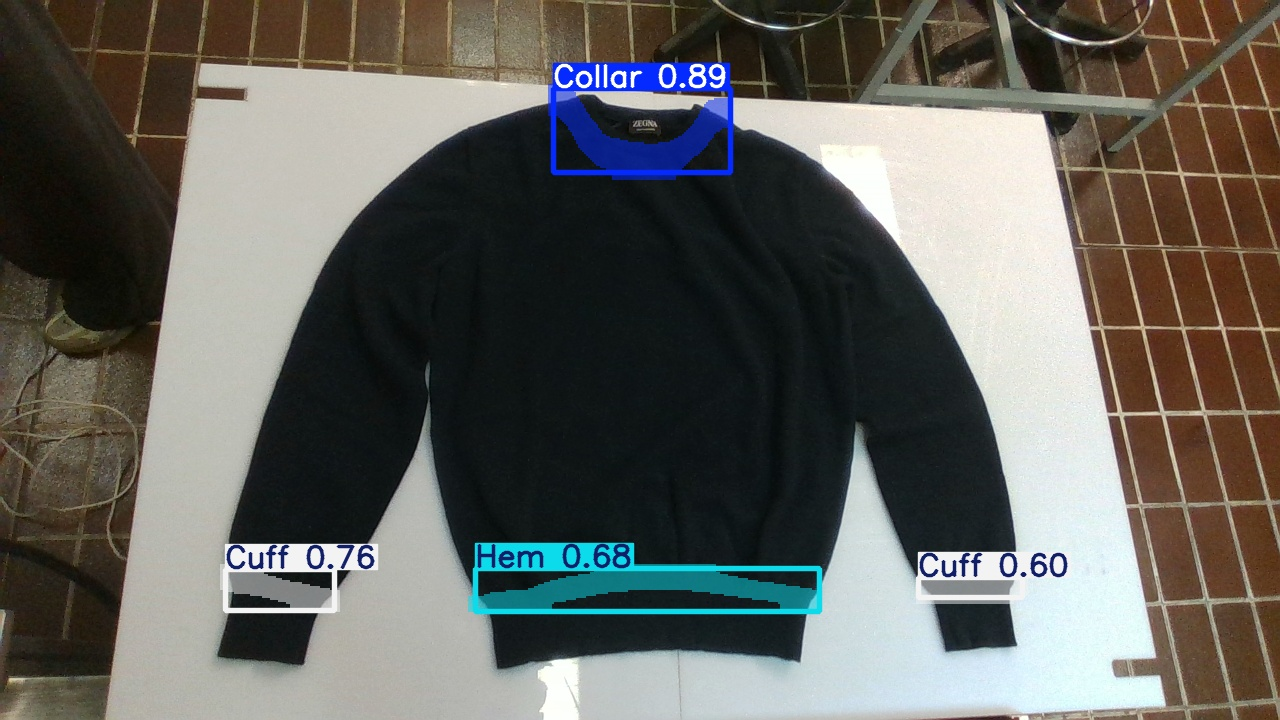
\includegraphics[width=\textwidth]{figures/inference_result.jpg}
        \caption{Box e maschere predette dalla rete}
        \label{fig:Maschere e box }
    \end{subfigure}
    \hfill % Spaziatura orizzontale tra le immagini
    % Seconda immagine
    \begin{subfigure}[b]{0.48\textwidth}
        \centering
        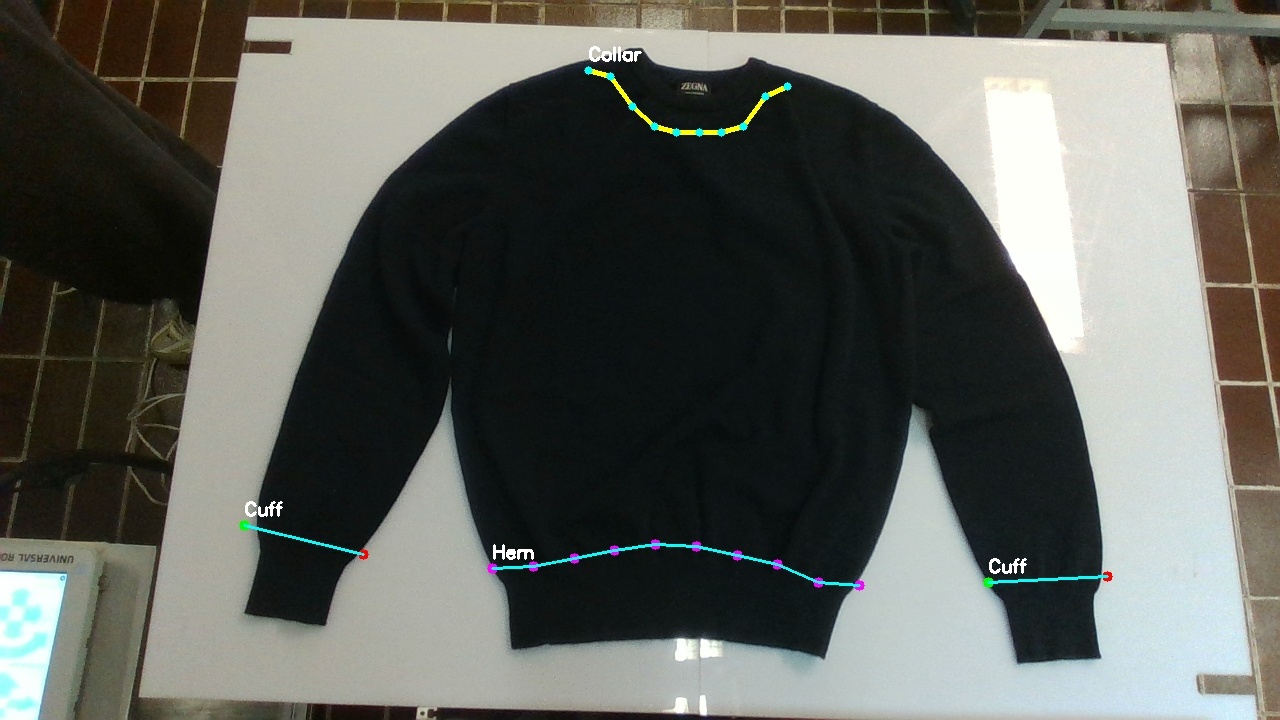
\includegraphics[width=\textwidth]{figures/inference_result_depth copy.jpg}
        \caption{Punti estratti dalle maschere predette dalla rete}
        \label{fig:Punti estratti}
    \end{subfigure}

    % Didascalia globale (opzionale)
    \caption{Confronto tra maschere predette e punti estratti}
    \label{fig:entrambe}
\end{figure}

Il modulo di pianificazione ha prodotto traiettorie cartesiane continue,
suddivise in segmenti di taglio e raccordi, interpolate con spline cubiche e
temporizzate con profili di velocità trapezoidali o triangolari. Le
posizioni, le velocità e gli orientamenti desiderati sono poi convertiti nello
spazio dei giunti mediante cinematica inversa differenziale con
Damped Least Squares.

Un risultato rilevante è stato il passaggio dal \textit{forward position
    controller} allo \textit{scaled joint trajectory controller}. L'invio punto
per punto dei riferimenti produceva leggeri scatti nel moto, mentre l'invio
dell'intera traiettoria come singolo goal \textit{FollowJointTrajectory} ha
reso l'esecuzione più fluida, delegando la temporizzazione al controller e
fornendo feedback, controllo delle tolleranze e scalatura rispetto ai limiti
imposti dal pendant. Infine, il launcher automatico ha eliminato
l'inserimento manuale delle coordinate, rendendo il ciclo completo
(home position, acquisizione, inferenza, esecuzione) avviabile con un unico
comando.

% TODO: inserire qui i risultati sperimentali effettivamente misurati
% (numero di prove, tasso di successo, errore di inseguimento, tempi).
% I valori attualmente presenti (20 maglioncini, 85\%, 20 ms, 1.2 s)
% devono essere riportati solo se supportati da misure reali.

\section{Limitazioni}

Il lavoro presenta alcune limitazioni che è opportuno evidenziare.

\begin{itemize}
    \item \textbf{Stima della profondità}: la distanza lungo l'asse z dei punti è affetta da rumore
          della mappa di profondità. Per questo la coordinata $z$ viene uniformata
          a una quota di riferimento calcolata sul fondomaglia. Si tratta di
          un'approssimazione geometrica che assume il capo sia posizionato su un piano.
    \item \textbf{Pianificazione in anello aperto sulla percezione}: i punti
          vengono estratti una sola volta dalla posa di \textit{home}, quindi eventuali spostamenti o
          deformazioni del capo dopo l'acquisizione non vengono rilevati.
\end{itemize}

\section{Sviluppi futuri}

Alla luce delle limitazioni emerse, i principali sviluppi possibili sono:

\begin{itemize}
    \item ampliare e diversificare il dataset (capi, colori, illuminazione) e
          migliorare la segmentazione, ad esempio con modelli più grandi o con
          acquisizioni da più punti di vista (\textit{multi-view});
    \item correggere la ricostruzione della quota con la superficie reale del
          capo, anziché con un piano, e verificare la calibrazione
          \textit{hand-eye} della telecamera;
    \item introdurre un controllo in retroazione visiva o una riacquisizione
          periodica, per compensare spostamenti e deformazioni del tessuto;
\end{itemize}

\section{Conclusioni}

Il progetto ha dimostrato la fattibilità di un approccio \textit{vision-guided}
per il taglio robotizzato di tessuti deformabili, integrando
segmentazione di istanze, ricostruzione 3D, pianificazione di traiettoria
e controllo di un manipolatore UR5 in un'architettura modulare basata su
ROS~2. L'uso di un ambiente di simulazione ha consentito di
validare in anticipo il modello cinematico, le trasformazioni tra i sistemi di
riferimento e la comunicazione tra i moduli, riducendo i tempi e i rischi
della sperimentazione sul robot reale. Le principali criticità, legate
all'incertezza percettiva, alla deformabilità del materiale e alla
precisione del controllo, restano aperte e indicano le direzioni di
approfondimento per sviluppi futuri.